\documentclass[11pt,twoside]{article}
\newif\ifproblem\newif\ifsolution\problemtrue
\newif\ifhw\hwtrue
\usepackage{exams}
\usepackage{pgf,tikz}
\usepackage{pgfplots,array}
\usepackage{tikz,graphicx,amsmath,amsfonts,amscd,amssymb,bm,cite,epsfig,epsf,url,color}
\examheadings
  {March}                          % Problem set date
  {March}           				% Solutions date
  {Midterm}
%% Probability operators and functions
%
% \def \P{\mathrm{P}}
\def \P{\mathrm{P}}
\def \E{\mathrm{E}}
\def \Var{\mathrm{Var}}
\let\var\Var
\def \Cov {\mathrm{Cov}} \let\cov\Cov
\def \MSE {\mathrm{MSE}} \let\mse\MSE
\def \sgn {\mathrm{sgn}}
\def \R {\mathbb{R}}
\def \C {\mathbb{C}}
\def \N {\mathbb{N}}
\def \Z {\mathbb{Z}}
\def \cV {\mathcal{V}}
\def \cS {\mathcal{S}}
\DeclareMathOperator*{\argmin}{arg\,min}
\DeclareMathOperator*{\argmax}{arg\,max}
\newcommand{\red}[1]{\textcolor{red}{#1}}
\newcommand{\blue}[1]{\textcolor{blue}{#1}}
\newcommand{\green}[1]{\textcolor{ForestGreen}{ #1}}
\newcommand{\fuchsia}[1]{\textcolor{RoyalPurple}{ #1}}

%
%% Probability distributions
%
%\def \Bern    {\mathrm{Bern}}
%\def \Binom   {\mathrm{Binom}}
%\def \Exp     {\mathrm{Exp}}
%\def \Geom    {\mathrm{Geom}}
%\def \Norm    {\mathcal{N}}
%\def \Poisson {\mathrm{Poisson}}
%\def \Unif    {\mathrm {U}}
%
\newcommand{\bdb}[1]{\textcolor{red}{#1}}

\newcommand{\ml}[1]{\mathcal{ #1 } }
\newcommand{\wh}[1]{\widehat{ #1 } }
\newcommand{\wt}[1]{\widetilde{ #1 } }
\newcommand{\conj}[1]{\overline{ #1 } }
\newcommand{\rnd}[1]{\tilde{ #1 } }
\newcommand{\rv}[1]{ \rnd{ #1}  }
\newcommand{\rx}{\rnd{ x}  }
\newcommand{\ry}{\rnd{ y}  }
\newcommand{\ra}{\rnd{ a}  }
\newcommand{\rb}{\rnd{ b}  }
\newcommand{\rpc}{\widetilde{ pc}  }

\def \cnd {\, | \,}
\def \Id { I }
\def \J {\mathbf{1}\mathbf{1}^T}

\newcommand{\op}[1]{\operatorname{#1}}
\newcommand{\setdef}[2]{ := \keys{ #1 \; | \; #2 } }
\newcommand{\set}[2]{ \keys{ #1 \; | \; #2 } }
\newcommand{\sign}[1]{\op{sign}\left( #1 \right) }
\newcommand{\trace}[1]{\op{tr}\left( #1 \right) }
\newcommand{\tr}[1]{\op{tr}\left( #1 \right) }
\newcommand{\inv}[1]{\left( #1 \right)^{-1} }
\newcommand{\abs}[1]{\left| #1 \right|}
\newcommand{\sabs}[1]{| #1 |}
\newcommand{\keys}[1]{\left\{ #1 \right\}}
\newcommand{\sqbr}[1]{\left[ #1 \right]}
\newcommand{\sbrac}[1]{ ( #1 ) }
\newcommand{\brac}[1]{\left( #1 \right) }
\newcommand{\bbrac}[1]{\big( #1 \big) }
\newcommand{\Bbrac}[1]{\Big( #1 \Big)}
\newcommand{\BBbrac}[1]{\BIG( #1 \Big)}
\newcommand{\MAT}[1]{\begin{bmatrix} #1 \end{bmatrix}}
\newcommand{\sMAT}[1]{\left(\begin{smallmatrix} #1 \end{smallmatrix}\right)}
\newcommand{\sMATn}[1]{\begin{smallmatrix} #1 \end{smallmatrix}}
\newcommand{\PROD}[2]{\left \langle #1, #2\right \rangle}
\newcommand{\PRODs}[2]{\langle #1, #2 \rangle}
\newcommand{\der}[2]{\frac{\text{d}#2}{\text{d}#1}}
\newcommand{\pder}[2]{\frac{\partial#2}{\partial#1}}
\newcommand{\derTwo}[2]{\frac{\text{d}^2#2}{\text{d}#1^2}}
\newcommand{\ceil}[1]{\lceil #1 \rceil}
\newcommand{\Imag}[1]{\op{Im}\brac{ #1 }}
\newcommand{\Real}[1]{\op{Re}\brac{ #1 }}
\newcommand{\norm}[1]{\left|\left| #1 \right|\right| }
\newcommand{\norms}[1]{ \| #1 \|  }
\newcommand{\normProd}[1]{\left|\left| #1 \right|\right| _{\PROD{\cdot}{\cdot}} }
\newcommand{\normTwo}[1]{\left|\left| #1 \right|\right| _{2} }
\newcommand{\normTwos}[1]{ \| #1  \| _{2} }
\newcommand{\normZero}[1]{\left|\left| #1 \right|\right| _{0} }
\newcommand{\normTV}[1]{\left|\left| #1 \right|\right|  _{ \op{TV}  } }% _{\op{c} \ell_1} }
\newcommand{\normOne}[1]{\left|\left| #1 \right|\right| _{1} }
\newcommand{\normOnes}[1]{\| #1 \| _{1} }
\newcommand{\normOneTwo}[1]{\left|\left| #1 \right|\right| _{1,2} }
\newcommand{\normF}[1]{\left|\left| #1 \right|\right| _{\op{F}} }
\newcommand{\normLTwo}[1]{\left|\left| #1 \right|\right| _{\ml{L}_2} }
\newcommand{\normNuc}[1]{\left|\left| #1 \right|\right| _{\ast} }
\newcommand{\normOp}[1]{\left|\left| #1 \right|\right|  }
\newcommand{\normInf}[1]{\left|\left| #1 \right|\right| _{\infty}  }
\newcommand{\proj}[1]{\mathcal{P}_{#1} \, }
\newcommand{\diff}[1]{ \, \text{d}#1 }
\newcommand{\vc}[1]{\boldsymbol{\vec{#1}}}
\newcommand{\rc}[1]{\boldsymbol{#1}}
\newcommand{\vx}{\vec{x}}
\newcommand{\vy}{\vec{y}}
\newcommand{\vz}{\vec{z}}
\newcommand{\vu}{\vec{u}}
\newcommand{\vv}{\vec{v}}
\newcommand{\vb}{\vec{\beta}}
\newcommand{\va}{\vec{\alpha}}
\newcommand{\vaa}{\vec{a}}
\newcommand{\vbb}{\vec{b}}
\newcommand{\vg}{\vec{g}}
\newcommand{\vw}{\vec{w}}
\newcommand{\vh}{\vec{h}}
\newcommand{\vnu}{\vec{\nu}}
\newcommand{\rvnu}{\vc{\nu}}

\newtheorem{theorem}{Theorem}[section]
% \declaretheorem[style=plain,qed=$\square$]{theorem}
\newtheorem{corollary}[theorem]{Corollary}
\newtheorem{definition}[theorem]{Definition}
\newtheorem{lemma}[theorem]{Lemma}
\newtheorem{remark}[theorem]{Remark}
\newtheorem{algorithm}[theorem]{Algorithm}

% \theoremstyle{definition}
%\newtheorem{example}[proof]{Example}
%\declaretheorem[style=definition,qed=$\triangle$,sibling=definition]{example}
%\declaretheorem[style=definition,qed=$\bigcirc$,sibling=definition]{application}

%
%% Typographic tweaks and miscellaneous
%\newcommand{\sfrac}[2]{\mbox{\small$\displaystyle\frac{#1}{#2}$}}
%\newcommand{\suchthat}{\kern0.1em{:}\kern0.3em}
%\newcommand{\qqquad}{\kern3em}
%\newcommand{\cond}{\,|\,}
%\def\Matlab{\textsc{Matlab}}
%\newcommand{\displayskip}[1]{\abovedisplayskip #1\belowdisplayskip #1}
%\newcommand{\term}[1]{\emph{#1}}
%\renewcommand{\implies}{\;\Rightarrow\;}

% My macros

\def\Kset{\mathbb{K}}
\def\Nset{\mathbb{N}}
\def\Qset{\mathbb{Q}}
\def\Rset{\mathbb{R}}
\def\Sset{\mathbb{S}}
\def\Zset{\mathbb{Z}}
\def\squareforqed{\hbox{\rlap{$\sqcap$}$\sqcup$}}
\def\qed{\ifmmode\squareforqed\else{\unskip\nobreak\hfil
\penalty50\hskip1em\null\nobreak\hfil\squareforqed
\parfillskip=0pt\finalhyphendemerits=0\endgraf}\fi}

%\DeclareMathOperator*{\E}{\rm E}
%\DeclareMathOperator*{\argmax}{\rm argmax}
%\DeclareMathOperator*{\argmin}{\rm argmin}
%\DeclareMathOperator{\sgn}{sign}
\DeclareMathOperator{\supp}{supp}
\DeclareMathOperator{\last}{last}
%\DeclareMathOperator{\sign}{\sgn}
\DeclareMathOperator{\diag}{diag}
\providecommand{\abs}[1]{\lvert#1\rvert}
\providecommand{\norm}[1]{\lVert#1\rVert}
\def\vcdim{\textnormal{VCdim}}
\DeclareMathOperator*{\B}{\textbf{B}}

%\DeclarePairedDelimiter\ceil{\lceil}{\rceil}
%\DeclarePairedDelimiter\floor{\lfloor}{\rfloor}

\newcommand{\cX}{{\mathcal X}}
\newcommand{\cY}{{\mathcal Y}}
\newcommand{\cA}{{\mathcal A}}
\newcommand{\ignore}[1]{}
\newcommand{\bi}{\begin{itemize}}
\newcommand{\ei}{\end{itemize}}
\newcommand{\be}{\begin{enumerate}}
\newcommand{\ee}{\end{enumerate}}
\newcommand{\bd}{\begin{description}}
\newcommand{\ed}{\end{description}}
\newcommand{\h}{\widehat}
\newcommand{\e}{\epsilon}
\newcommand{\mat}[1]{{\mathbf #1}}
%\newcommand{\R}{\mat{R}}
\newcommand{\0}{\mat{0}}
\newcommand{\M}{\mat{M}}

\newcommand{\D}{\mat{D}}
\renewcommand{\r}{\mat{r}}
\newcommand{\x}{\mat{x}}
\renewcommand{\u}{\mat{u}}
\renewcommand{\v}{\mat{v}}
\newcommand{\w}{\mat{w}}
\renewcommand{\H}{\text{0}}
\newcommand{\T}{\text{1}}
%\newcommand{\set}[1]{\{#1\}}
\newcommand{\xxi}{{\boldsymbol \xi}}
\newcommand{\ssigma}{{\boldsymbol \sigma}}
\newcommand{\Alpha}{{\boldsymbol \alpha}}
\newcommand{\tts}{\tt \small}
\newcommand{\hint}{\emph{hint}}
\newcommand{\matr}[1]{\bm{#1}}     % ISO complying version
\newcommand{\vect}[1]{\bm{#1}} % vectors

%\newcommand{\Var}{\mathrm{Var}}
%\newcommand{\Cov}{\mathrm{Cov}}

% New commands
\newcommand{\SP}{\mathbf{S}_{+}^n}
\newcommand{\Proj}{\mathcal{P}_{\mathcal{S}}}
\DeclarePairedDelimiterX{\inp}[2]{\langle}{\rangle}{#1, #2}
\newtheorem{proof}{Proof}


\begin{document}

\examheader

\ifproblem
\begin{center}
\vspace{-26pt} % kludge
\advance\textwidth -1.6in
\medskip
\end{center}
\fi
% Write the answer to each problem \underline{in a separate sheet of paper}.\\

Justify all your answers. Full credit will \underline{not be given} to any answer that is not adequately justified. You can use results from the notes and other material as long as you explain why they apply.

\textbf{You are not allowed to communicate with anyone about the midterm while you are doing it.} We have preferred to prioritize making your life as easy as possible from the logistical point of view, instead of making the timing very tight to avoid cheating. Please don't abuse this. It is not fair to your fellow students.

Submit the midterm through Gradescope, just like the homework. Please remember to start each problem on a separate page (just like the homework).

\begin{exam}


%%%%%%%%%%%%%%%%%%%%%%%%%%%%%%%%%%%%%
%%%%%%%%%%%%%%%%%%%%%%%%%%%%%%%%%%%%%
\item
\begin{exercise}[Short questions (\emph{20 points}).]
\begin{problem}

\begin{enumerate}
\item We are interested in clustering these 2D data. Is PCA the right way of performing dimensionality reduction to 1D for this task? (5 points)\\

\medskip
Doing PCA we will select the horizontal axis as the first principal direction since most of the variance of the data is explained by projecting along this axis but then we will not be able to separate the initial two clusters which were 
separated clearly in 2D. So PCA is not the  right way of performing dimensionality reduction to 1D for this task.

\begin{center}
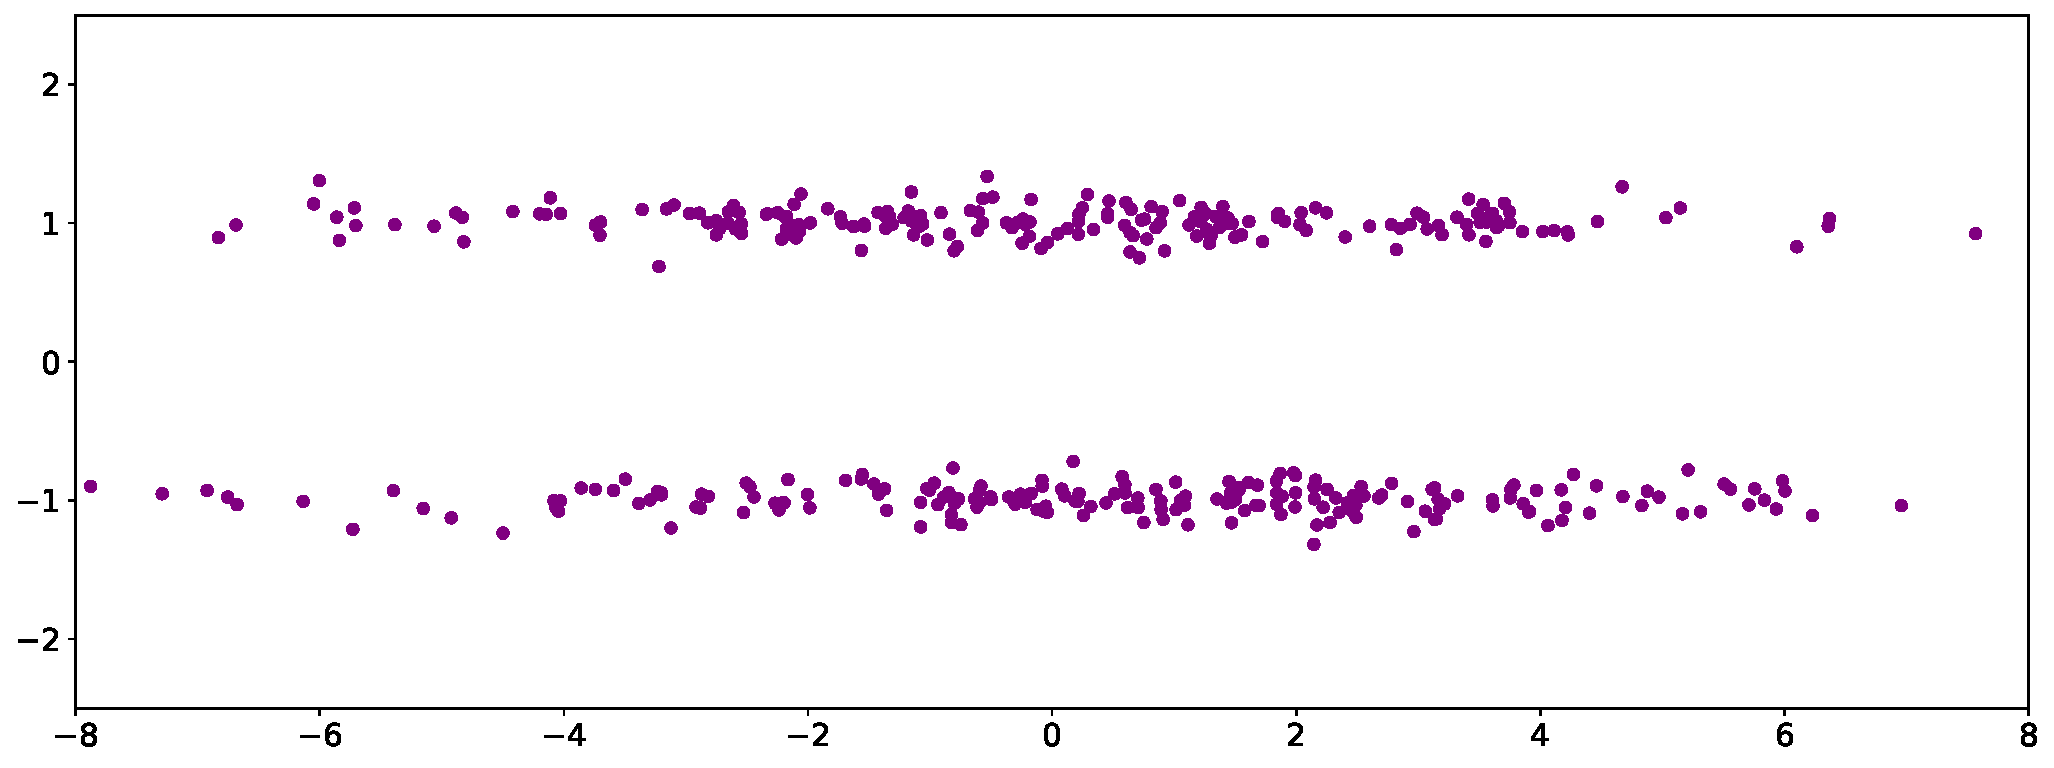
\includegraphics[width=.75\linewidth]{figs/clustering_PCA.pdf}
\end{center}
\item We are interested in computing the singular values of a matrix $A \in \R^{p \times p}$, but we cannot observe it directly. We can only observe its output for some inputs of our choice. A popular technique in such settings is to choose random inputs. Explain how to compute the singular values of $A$ from the random vector $\rnd{y}:=A \rnd{x}$, where $\rx$ is a zero mean random vector with covariance matrix equal to the identity.  (5 points)\\

Using theorem 8.6 from PCA notes, we  have $\Sigma_{\ry} = A \Sigma_{\rx} A^T = A A^T$, then with random inputs we can build the covariance matrix using its outputs, which is a square matrix.
We can then perform an eigendecomposition which gives us the eigenvalues of $AA^T$, which is positive definite, the singular value of $A$ which are non negative will be the square roots of these eigenvalues.


\item Explain how performing PCA on the feature matrix of a linear regression problem can help you decide whether to apply OLS or ridge regression.  (5 points)

Performing PCA on the feature matrix gives us the eigenvalues of the covariance matrix and if some eigenvalues are very small compared to the others, it is the sign of correlations between features.
Then the covariance matrix might be not full rank and the OLS estimator coefficients might blow up, also the small singular values might cause high variance of the OLS coefficients if there is not a lot of samples.
We might want then decide to use ridge regression instead to neutralize the high variances due to the small singular values.

\item For a fixed feature matrix and a fixed response vector, can the training error of OLS be larger than the training error of ridge regression for some value of the regularization parameter $\lambda>0$?  (5 points)

if we compare OLS and ridge regression training errors:
$$\text{OLS} = \min \big\| \begin{bmatrix} y  - X^T \beta  \end{bmatrix}\big\|_2^2$$

$$\text{RR} = \min \big\| \begin{bmatrix} y  - X^T \beta  \\  \sqrt{\lambda} I \end{bmatrix}\big\|_2^2$$

\begin{align*}
	\big\| \begin{bmatrix} y  - X^T \beta  \end{bmatrix}\big\|_2^2 \le  \big\| \begin{bmatrix} y  - X^T \beta  \\  \sqrt{\lambda} I \end{bmatrix}\big\|_2^2 
	= \big\| \begin{bmatrix} y  - X^T \beta  \end{bmatrix}\big\|_2^2  +  \lambda \big\|  I \big\|_2^2 
\end{align*}
Taking the minimum on both sides shows that for any $\lambda > 0$, we have that the training error of OLS cannot be  larger than the training error of ridge regression.

\end{enumerate}

\end{problem}

\end{exercise}

\newpage

\item
\begin{exercise}[Normalization (\emph{30 points}).]
\begin{problem}
In this problem we study the effect of normalizing by the standard deviation before performing principal component analysis. Let $\rx$ be a zero-mean $3$-dimensional random vector with covariance matrix 
\begin{align}
\Sigma_{\rx} := \MAT{ 100 & 25 & 0 \\ 25 & 400 & 0 \\ 0 & 0 & 0.16 }.
\end{align}
We define the normalized vector $\ry$ as
\begin{align}
\ry[i] := \frac{ \rx[i]}{ \sqrt{\var (\rx[i])}} \quad 1 \leq i \leq 3.
\end{align}
\begin{enumerate}
\item Compute the covariance matrix of $\ry$.  (10 points)
\begin{align*}
	\var(\ry[i] )	&=	\var(\frac{ \rx[i]}{ \sqrt{\var (\rx[i])}})  \quad 1 \leq i \leq 3\\
			&= \frac{1}{\var (\rx[i]) } \var (\rx[i]) \\
			&= 1 \\
	\Cov({\ry[i] }{\ry[j]})	&= \Cov({\frac{ \rx[i]}{ \sqrt{\var (\rx[i])}}} {\frac{ \rx[j]}{ \sqrt{\var (\rx[j])}}}) \; i \neq j  \; \quad 1 \leq i,j \leq 3\\
					&= \frac{1} { \sqrt{\var (\rx[i]) \var (\rx[j])  }} \Cov( {\rx[i]} {\rx[j]}) \\
\end{align*}

Using the covariance of $\rx$ we obtain the covariance of $\ry$:
\begin{align}
\Sigma_{\ry} := \MAT{ 1 & 0.125 & 0 \\ 0.125 & 1 & 0 \\ 0 & 0 & 1 }.
\end{align}

\item Is the directional variance of $\ry$ equal to one in every direction?  (5 points)
The directional variance will be the same in every direction if we have for covariance of $\ry$ the identity matrix which is not the case, so it is not the same in every direction.

\item We decide to reduce the dimensionality of $\rx$ and $\ry$ to two dimensions using PCA. Report what directions are selected for each of the random vectors. (Feel free to use a computer for your calculations, but explain what you are doing.)  (10 points)
We perform the eigendecomposition of the covariance of $\rx$ and found its eigenvalues and eigenvectors:
\begin{align*}
	\Sigma_{\rx}	&=	U_x D_x U_x^T \\
	D _x			&= \MAT{0.16 & 0  & 0 \\ 0 & 97.93  & 0 \\ 0 & 0 & 402.06} \\
				&= [\lambda_3 \; \lambda_2 \; \lambda_1 ] \\
	U_x 			&= \MAT{ 0 & -0.996 &  0.0824 \\  0 & 0.0824 & 0.996 \\  1 & 0 & 0 } \\
				&= [u_3 \; u_2 \; u_1 ]
\end{align*}
Using theorem 6.1 from the PCA notes the first eigenvector $u_1$ is the direction of highest variance, which is equal to corresponding eigenvalue $\lambda_1$.
In directions orthogonal to $u_1$  the maximum variance is attained by the second eigenvector $u_2$, and equals the corresponding eigenvalue  $\lambda_2$.
And the last eigenvalue $0.16$ is very small compared to the two others  so most of the variance is captured by the two eigenvectors $u_1$ and $u_2$.
If we project the data using  the two eigenvectors $u_1$ and $u_2$ we will reduce the dimensions from three to two while conserving most of the variance.
Also as a result of theorem7.1 from PCA notes, projection along these directions achieves the highest variances compared to any other directions.

Similarly for $\ry$ we compute the eigendecomposition of its covariance matrix and find:
\begin{align*}
	\Sigma_{\ry}	&=	U_y D_y U_y^T \\
	D _y			&= \MAT{0.875 & 0  & 0 \\ 0 & 1  & 0 \\ 0 & 0 & 1.125} \\
				&= [\mu_3 \; \mu_2 \; \mu_1 ] \\
	U_y			&= \MAT{ -0.7071 & 0 &  0.7071 \\  0.7071 & 0 & 0.7071 \\  0 & 1 & 0 } \\
				&= [v_3 \; v_2 \; v_1 ]
\end{align*}
Using theorem 6.1 from PCA notes, we select for directions $v_1$ and $v_2$ corresponding to the largest two eigenvalues and project the data along these two directions.


\item Explain which of the two options for dimensionality reduction to 2D would make more sense in each of the following situations and why that is the case: (1) The entries of $\rx$ represent the weight (in kilograms), heart rate (in beats per minute), and height (in meters) of a set of hospital patients. (2) The entries of $\rx$ represent the length, width and height (all in centimeters) of a set of cars.  (5 points)


If you compare the eigenvalues of $\Sigma_{\rx}$ there is a large difference between the last two eigenvalues  and the first one and less differences between the eigenvalues of  $\Sigma_{\ry}$.
For the first case the variables have very different scales compared to the variables related to a set of cars, so it will make sense to use the directions of the PCA on $\Sigma_{\ry}$ to perform dimensionality reduction to 2D 
for the dataset related to hospital patients so one variable like height, does not dominate the two others. And we will do dimension reduction using  the directions of PCA on $\Sigma_{\rx}$ for the data related to 
the length, width and height (all in centimeters) of a set of cars.


\end{enumerate}

\end{problem}

\end{exercise}

\newpage

\item
\begin{exercise}[Noise cancellation (\emph{20 points}).] 
\begin{problem} 
We are interested in recording the voice of a pilot in a helicopter. To this end we place a microphone inside his helmet and another microphone outside. We model the measurements as
\begin{align}
\rx[1] & = \ry + \alpha \rnd{z}\\
\rx[2] & = \alpha \ry + \rnd{z},
\end{align}
where $\ry$ is a random variable modeling the voice of the pilot, $\rnd{z}$ is a random variable modeling the noise in the helicopter, and $0 < \alpha < 1$ is a constant that models the effect of the helmet. From past data, we determine that $\ry$, and $\rnd{z}$ are zero mean and uncorrelated with each other. The variances of $\ry$  and $\rnd{z}$ are equal to $1$ and 100 respectively.
\begin{enumerate}
\item Compute the best linear estimator of $\ry$ given $\rx[1]$ in terms of MSE, and the corresponding MSE, as a function of $\alpha$. Describe in words what the estimator does.  (10 points)\\

By independence
\begin{align*}
	\var(\rx[1])			&=	\var(\ry) + \var(\alpha \rnd{z}) \\
					&=	1 + \alpha^2	\var(\rnd{z}) \\
					&=	1 + 100 \alpha^2 \\
	\Sigma_{\rx[1]}		&=	1 + 100 \alpha^2 \\
	\Cov({\ry}{(\rx[1])})	&=	\E[ {\ry}{(\rx[1])} ] \\
					&=.  \var({\ry}) \\
					&=	1 \\
\end{align*}
By theorem 2.3 in linear regression notes, the estimate equals:
$$
		\hat{y}(\rx[1]) = \frac{\rx[1]} {100 \alpha^2 + 1}
$$
And the corresponding MSE equals:
\begin{align*}
	\E( (\hat{y}(\rx[1])  - \ry)^2 ]		&= \var(\ry) - \frac{1} {1 + 100 \alpha^2} \\
								&= 1 - \frac{1} {1 + 100 \alpha^2} \\
								&= \frac{100 \alpha^2}  {100 \alpha^2 + 1} 
\end{align*}
If $\alpha=0$ the estimate is the the voice of the pilot and when $\alpha \rightarrow 1$ then the estimate shrinks the voice of the pilot from the microphone.
$\alpha$ controls how much shrinkage we want of the voice of the pilot.

\item Compute the best linear estimator of $\ry$ given $\rx$ in terms of MSE, and the corresponding MSE, as a function of $\alpha$. Describe in words what the estimator does.  (10 points)
By independence
\begin{align*}
	\var(\rx[1])			&=	100 \alpha^2 + 1 \\
	\var(\rx[2])			&=	\var(\alpha \ry ) + \var(\rnd{z}) \\
					&=	 \alpha^2 + 100 \\
	\Cov({\rx[1]}{\rx[2]})	&=	\E[ (\ry + \alpha \rnd{z}) (\alpha \ry + \rnd{z}) ] \\
					&=	 \alpha E[\ry^2] + \alpha \E[\rnd{z})] \\
					&=	101 \alpha \\
	\Sigma_{\rx}		&= 	\MAT{100 \alpha^2 + 1 & 101 \alpha \\ 101 \alpha &  \alpha^2 + 100 } \\
	\Cov({\ry}{(\rx[1])})	&= 1 \\
	\Cov({\ry}{(\rx[2])})	&=	 \E[ \ry (\alpha \ry + \rnd{z}) ] \\
					&=	\alpha \E[\ry^2] = \alpha \\
	\Sigma_{\ry}		&=	\MAT{1 \\ \alpha}	\\			
\end{align*}
By theorem 2.3 in the linear regression notes, the estimate equals:
\begin{align*}
		\hat{y}(\rx) 	&= 	\rx^T 	\MAT{100 \alpha^2 + 1 & 101 \alpha \\ 101 \alpha &  \alpha^2 + 100 }^{-1}	\MAT{1 \\ \alpha} \\
					&= 	\frac{\rx[1] - \rx[2]} {1 - \alpha^2}
\end{align*}

And the corresponding MSE equals:
\begin{align*}
	\E( (\hat{y}(\rx)  - \ry)^2 ]		&= \var(\ry) - \MAT{1 \; \alpha} \MAT{100 \alpha^2 + 1 & 101 \alpha \\ 101 \alpha &  \alpha^2 + 100 }^{-1}	\MAT{1 \\ \alpha} \\
							&= 1 - \frac{\alpha -1} {\alpha^2-1} \\
							&= \frac{\alpha} {\alpha +1}
\end{align*}
The estimate as $\alpha \rightarrow 1$ approximatively cancels out the noise in a way that is optimal with respect to MSE, and provides better recording of the voice of the pilot.

\end{enumerate}
\end{problem} 
\end{exercise} 

\newpage

\item
\begin{exercise}[Adversarial perturbation (\emph{30 points}).] 
\begin{problem} 
Designing adversarial perturbations is an active area of research in deep learning. Here we study adversarial perturbations for linear regression. 
\begin{enumerate}
\item Let $\beta_{\op{OLS}}$ be the OLS coefficient estimate corresponding to a linear-regression problem where $X \in \R^{p \times n}$ is the feature matrix and $y \in \R^{n}$ is the response vector. We assume that $X$ is full rank and $p<n$. Your goal is to choose a noise vector $z \in \R^n$ with bounded $\ell_2$ norm ($\normTwos{z}\leq \gamma$ for a constant $\gamma > 0$) that will be added to $y$. Explain how to compute the $z$ that produces the maximum possible perturbation (in $\ell_2$ norm) to the OLS coefficient estimate, i.e. 
\begin{align}
z^{\op{adv}}_{\op{OLS}}:= \arg \max_{\normTwo{z} \leq \gamma} \normTwo{\beta_{\op{OLS}} - \beta^{\op{mod}}_{\op{OLS}}(z)}^2, \quad  \beta^{\op{mod}}_{\op{OLS}}(z) := \arg \min_{\beta} \normTwo{y+z - X^T\beta}^2.
\end{align}\\

Using theorem 2.4 from linear regression notes, we have 
$$
	 \beta^{\op{mod}}_{\op{OLS}}(z) = ( X X^T)^{-1} X (y + z)
$$
Let $X=U S V^T$ then 
\begin{align*}
	 \beta^{\op{mod}}_{\op{OLS}}(z)				&= ( U S V^T V S U^T)^{-1} U S V^T (y + z) \\
	 										&= U S^{-2} U^T U S V^T (y + z) \\
											&= U S^{-1} V^T (y + z) \\
	\beta_{\op{OLS}} - \beta^{\op{mod}}_{\op{OLS}}	&= U S^{-1} V^T z \\
											&= \sum_{i=1}^p	\frac{v_i^T z} {s_i} u_i \\
	 \arg \max_{\normTwo{z} \leq \gamma} \normTwo{\beta_{\op{OLS}} - \beta^{\op{mod}}_{\op{OLS}}(z)}^2
											&= \arg \max_{\normTwo{z} \leq \gamma} \|  U S^{-1} V^T z  \|_2^2 \\
											&=\arg \max_{\normTwo{z} \leq \gamma}  z^T V S^{-2} V^T z \\
\end{align*}

%If we choose a Gaussian vector of mean $0$  and unit variance then the vector $U S^{-1} V^T z$ is a Gaussian vector of dimension $p$ and covariance matrix $\Sigma = U S^{-1} V^T \Sigma_z V S^{-1} U^T = U S^{-2} U^T$.
%The norm of this vector therefore equals to the square l2 norm of an iid Gaussian random vector of dimension $p$, the expected value of its square l2 norm is, using theorem 4.5 from the PCA notes, $\sigma^2 p$.

By theorem 3.1 from linear regression notes,
 the optimal noise vector is the vector corresponding to the last row of $V$, $z=V[:,p]$, which matches the largest singular value of  $S^{-1}$ which is $\frac{1}{s_n}$ where
 $s_n \le \ldots \le s_1$ are the singular values of $X$. $z$ being the last right-singular vector has unit norm.
 With this value of $z^{\op{adv}}_{\op{OLS}}$, $\normTwo{\beta_{\op{OLS}}  - \beta^{\op{mod}}_{\op{OLS}}(z^{\op{adv}}_{\op{OLS}} ) }^2 = \frac{1}{s_n}$.

 (10 points)
\item Let $\rnd{x}_{\op{test}}$ be a random test feature vector. Consider the perturbation to the test prediction $x_{\op{test}}^T\beta(z_{\op{adv}}) - x_{\op{test}}^T\beta_{\op{OLS}}$ achieved by your choice in the previous question. Do you expect the variance of this perturbation to be larger if $\frac{1}{n}XX^T$ is a good approximation to the covariance matrix of $\rnd{x}_{\op{test}}$, or if it is not a good approximation? Why?
 (5 points)\\
 Using the theorem 4.8 from the PCA notes, we find
 $$
 	\var(\rnd{x}_{\op{test}}^T (\beta(z_{\op{adv}}) - \beta_{\op{OLS}}) ) = \sum_{i=1}^p \frac{u_i^T \Sigma_{\rnd{x}_{\op{test}}} u_i}{s_i^2}
 $$
 If this sample variance is a good approximation to the variance of the test data in that direction then
 $$
	 \var(\rnd{x}_{\op{test}}^T (\beta(z_{\op{adv}}) - \beta_{\op{OLS}}) ) \approx \frac{p}{n}
 $$
 If it is not a good approximation then the sample covariance matrix may not provide a good estimate of the feature variance in every direction, 
 in that case, there may be terms in the variance where $s_i$ is very small, due to correlations between the features, the variance of this perturbation will be larger.


\item Assume that the regularization parameter $\lambda > 0$ is known to you. Explain how to choose the $z$ that produces the maximum possible perturbation (in $\ell_2$ norm) to the ridge regression coefficient estimate, i.e. 
\begin{align}
z^{\op{adv}}_{\op{RR}}(\lambda) := \arg \max_{\normTwo{z} \leq \gamma} \normTwo{\beta_{\op{RR}}(\lambda) - \beta^{\op{mod}}_{\op{RR}}(z,\lambda)}^2, \quad  \beta^{\op{mod}}_{\op{RR}}(z,\lambda) := \arg \min_{\beta} \normTwo{y+z - X^T\beta}^2+\lambda \normTwo{\beta}^2. \notag
\end{align}
Is the perturbation $\normTwo{\beta_{\op{RR}}(\lambda) - \beta^{\op{mod}}_{\op{RR}}(z^{\op{adv}}_{\op{RR}}(\lambda),\lambda) }^2$ larger or smaller than the one achieved for OLS in the previous question, $\normTwo{\beta_{\op{OLS}}  - \beta^{\op{mod}}_{\op{OLS}}(z^{\op{adv}}_{\op{OLS}} ) }^2$?  (10 points)\\

Using theorem 5.2 from linear regression notes, we have 
\begin{align*}
	\beta_{\op{RR}}(\lambda)										&=	(X X^T + \lambda I)^{-1} X y \\
	\beta^{\op{mod}}_{\op{RR}}(z,\lambda) 							&= 	(X X^T + \lambda I)^{-1} X (y + z) \\
	\beta_{\op{RR}}(\lambda)	 -  \beta^{\op{mod}}_{\op{RR}}(z,\lambda)		&= 	(X X^T + \lambda I)^{-1}  X z \\
															&= 	(U S V^T V S U^T + \lambda UU^T) ^{-1}  X z \\
															&=    U (S^2 + \lambda I)^{-1} U^T U S V^T z \\
															&= 	U  (S^2 + \lambda I)^{-1}  S V^T z \\
															&= 	\sum_{i=1}^p	\frac{s_i \PROD{v_i}{z}} {s_i^2 + \lambda} u_i \\ 
 \arg \max_{\normTwo{z} \leq \gamma} \normTwo{\beta_{\op{RR}}(\lambda) - \beta^{\op{mod}}_{\op{RR}}(z,\lambda)}^2 &=
 								 \arg \max_{\normTwo{z} \leq \gamma}   |\| U  (S^2 + \lambda I)^{-1}  S V^T z  \|_2^2 \\	
								 &=  \arg \max_{\normTwo{z} \leq \gamma}  z^T V^T (S^2 + \lambda I)^{-2} S^2 V^T z	\\						
\end{align*}
For a fixed $\lambda > 0$, $z$ will be the right singular vector $v_i$, corresponding to the largest entry $\frac{s_i} {s_i^2 + \lambda}$.
Setting $\lambda = 0$ we have the same perturbation as the perturbation obtained in part a, and as $\lambda \rightarrow \infty$, the maximum perturbation to the ridge regression coefficient estimate goes to $0$.
The difference between the two perturbations is $\frac{1} {s_n} - \frac{s_i} {s_i^2 + \lambda}$ which could be positive or negative depending the values of the singular values.


\item How would you set $\lambda$ to minimize the $\ell_2$ norm of the adversarial perturbation, $\normTwo{\beta_{\op{RR}}(\lambda) - \beta^{\op{mod}}_{\op{RR}}(z^{\op{adv}}_{\op{RR}}(\lambda),\lambda) }^2$? Is this a reasonable approach?  (5 points)\\

The perturbation is minimized by increasing $\lambda$. 
Increasing $\lambda$ reduces the  adversarial perturbation, but as described in the PCA notes in the chapter about ridge regression, too large values for $\lambda$ reduces the ridge regression coefficients estimates, which become eventually too small
to produce an accurate fit. There is a trade-off to achieve and it is determined using cross-validation.

 \end{enumerate}

\end{problem}

\end{exercise}


\end{exam}
\end{document}
